\documentclass[aspectratio = 169]{chariteBeamer}
\usepackage[english]{babel} %% english
\usepackage[utf8]{inputenc}
\usepackage[T1]{fontenc}
\usepackage{hyperref}
\usepackage{blkarray}
\tikzset{>=latex}
\usepackage[edges]{forest}
\usetikzlibrary{positioning}
\usepackage{biostat}
\setbeamertemplate{caption}[numbered]
\let\qed\relax
\forestset{declare toks={elo}{}}
\graphicspath{{figures/}}
%% ================================================================== %% 

\author[L. Mödl, M. Becher, E. Sprünken]{Lukas Mödl, Matthias Becher, Erin Sprünken} 
\title{Day 3 -- Statistical Tests and Regression}
\place{R-Course}
\date[]{Updated: \today}
\email{biometrie-rkurs@charite.de} 

%% ================================================================== %% 

\hyphenation{Sam-ples}
\begin{document}

\begin{frame}[plain]
    \titlepage%
\end{frame}
\frame{\tableofcontents}


\section{Statistical Tests}

\begin{frame}[fragile]{Statistische Tests in R}
	\begin{itemize}
		\item t-Test = \verb+t.test()+
		\item Chi-Square Test = \verb+chisq.test()+
		\item Wilcoxon-Mann-Whitney-Test = \verb+wilcox.test()+
		\item Fisher Test = \verb+fisher.test()+
		\item McNemar's Test = \verb+mcnemar.test()+
		\item Binomial Test = \verb+binom.test()+
		\item ...
	\end{itemize}
\end{frame}


\begin{frame}[fragile]{t-Test}
\verb+t.test(x,...)+\\
Parameter:
	\begin{itemize}
		\item x = A data vector
		\item y = An optional second vector (e.g. for two-sample problems)
		\item alternative = c("two.sided", "less", "greater")
		\item mu = Assumed mean under the null hypothesis
		\item paired = c(TRUE, FALSE)
	\end{itemize}
\end{frame}

\begin{frame}[fragile]{Example t-Test:}	
	\begin{center}
		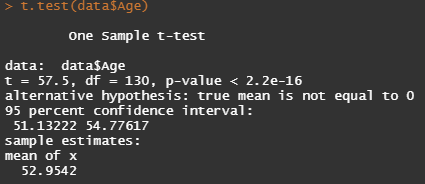
\includegraphics{OneSampleTtest}
	\end{center}
\end{frame}

\begin{frame}[fragile]{Example t-Test:}	
	\begin{center}
		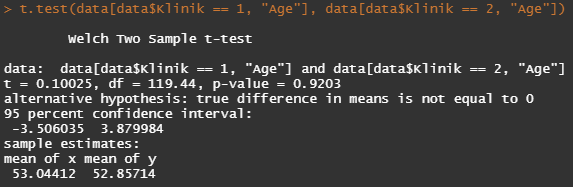
\includegraphics{TwoSampleTtest}
	\end{center}
Remark: R assumes unequal variances per default
\end{frame}

\begin{frame}[fragile]{Chi-Square Test:}	
	\verb+chisq.test()+ \\

	Beispiel: \\
	\begin{columns}[T]
		\begin{column}{0.5\textwidth}
			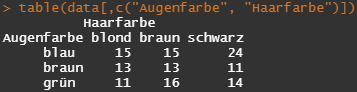
\includegraphics[width=7.5cm]{tabledata}
		\end{column}
		\begin{column}{0.5\textwidth}
			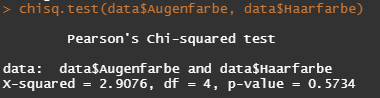
\includegraphics[width=7.5cm]{chisq}
		\end{column}
	\end{columns}
\end{frame}


%% ================================================================== %%
\section{Regression Analysis}

\begin{frame}[fragile]{Formulas in R}
	To conduct a regression we have to tell R, which columns of our data are independent variables and which is the dependent one. For this we have formulas:
	\begin{itemize}
		\item Only certain variables shall be used:
			\begin{center}
				Y\textasciitilde X1 + X2 + X3 + ... 
			\end{center}
		\item All variables from the data shall be used:
			\begin{center}
				Y\textasciitilde.
			\end{center}
	\end{itemize}
\end{frame}



\begin{frame}[fragile]{Linear Regression}
	\begin{itemize}
		\item \verb"model <- lm(Weight~Age+Sex+Height+Klinik, data =data)"
		\item \verb+summary(model)+
		\item Remark: "0 +" at the beginning of the right-hand-side leads to omission of the intercept
	\end{itemize}
			
	\begin{center}
		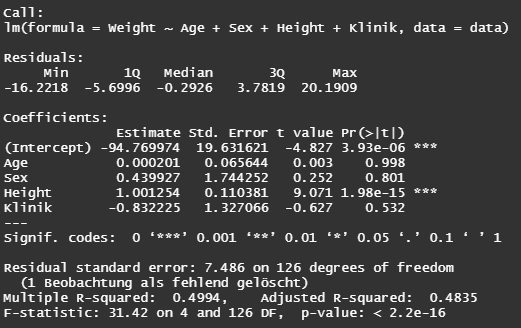
\includegraphics[height=3.75cm]{LinearRegressionSummary}
	\end{center}
\end{frame}

\begin{frame}[fragile]{Linear Regression Plot}
	\begin{columns}[T]
		\begin{column}{0.6\textwidth}
			\begin{itemize}
				\item \verb+plot(data$Height,data$Weight)+
				\item \verb+abline(model)+
			\end{itemize}
		\end{column}
		\begin{column}{0.4\textwidth}
			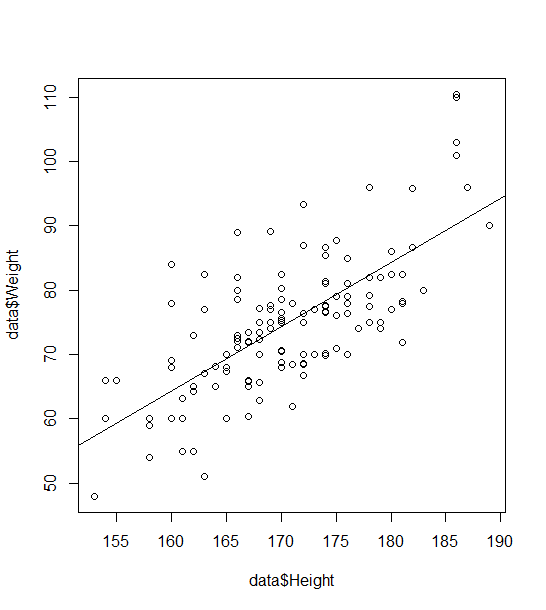
\includegraphics[height=6.5cm]{LinearRegressionPlot}
		\end{column}
	\end{columns}
\end{frame}

\begin{frame}[fragile]{Logistic Regression}
	\begin{itemize}
		\item \verb+model <- glm(y~., data = logistic_data, family = binomial)+
		\item \verb+summary(model)+
	\end{itemize}
			
	\begin{center}
		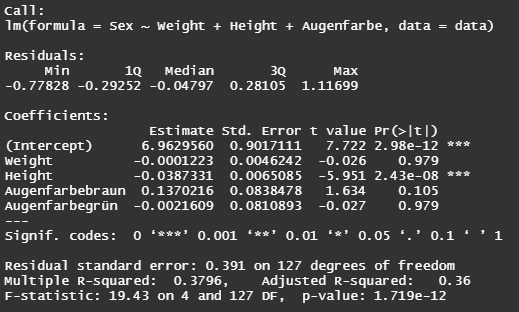
\includegraphics[height=4cm]{LogisticRegressionSummary}
	\end{center}
\end{frame}

\begin{frame}[fragile]{One-Way ANOVA}
	\begin{itemize}
		\item \verb+model <- aov(formula, data)+
	\end{itemize}	
	\begin{center}
		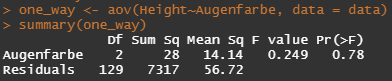
\includegraphics{OneWay}
	\end{center}
\end{frame}

\begin{frame}[fragile]{Two-Way ANOVA}
	\begin{center}
		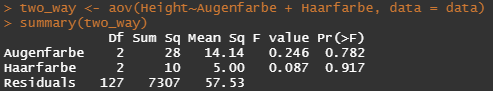
\includegraphics{TwoWay}
	\end{center}
\end{frame}

\begin{frame}[fragile]{Interaction ANOVA}
	\begin{center}
		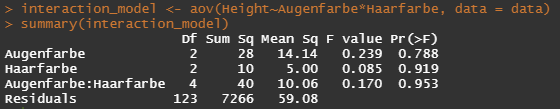
\includegraphics{Interaction}
	\end{center}
\end{frame}




%% ================================================================== %%

	


\section{\textsf R Packages}


\begin{frame}[fragile]{Installing further \textsf R Packages}
    Every \textsf R Environment installs and loads by default the packages \texttt{base}, \texttt{stats}, \texttt{datasets}, \texttt{methods} and \texttt{graphics}.\bigskip
    \begin{itemize}
        \item Installation of further packages:
        \begin{verbatim}
        install.packages("name-of-package", dependencies = TRUE)
        \end{verbatim}
        \item At the start R any package, which shall be used, must be loaded:
        \begin{verbatim}
        library("name-of-package")
        \end{verbatim}
        \item Updating of packages:
        \begin{verbatim}
        update.packages()
        \end{verbatim}
    \end{itemize}
\end{frame}

\begin{frame}[fragile]{Example: Installing and Loading of the \textsf R Package \texttt{MASS}}
    \begin{center}
        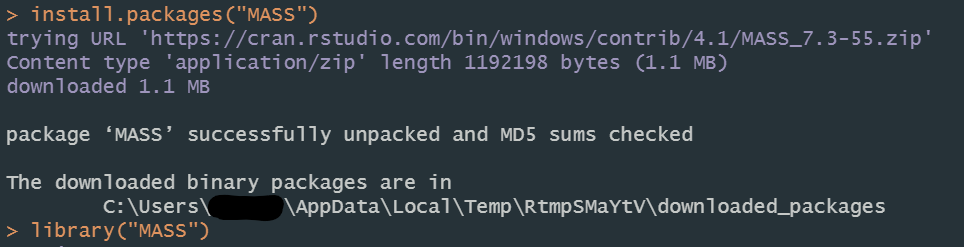
\includegraphics[width=\textwidth, keepaspectratio]{pakete.png}
    \end{center}
\end{frame}


\begin{frame}[fragile]{Useful packages}
	\begin{itemize}
		\item \verb+MatchIt+ for Propensity Score Matching 
	          \item \verb+MASS+ for Negative-binomial Regression
	          \item \verb+lmer+ and \verb+lme4+ for Mixed-Models 
	          \item \verb+pwr+ for Power-Analysis and especially sample size planning
	          \item \verb+ggplot2+ for nice plots
	          \item \verb+haven+ to read \verb+.sav+-Files (SPSS)
	          \item ...
	\end{itemize}
\end{frame}
	



\end{document}
%% ================================================================== %%
%% ================================================================== %% 
